\documentclass[11pt]{standalone}
\usepackage{amssymb}
\usepackage{amsmath}
\usepackage[no-math]{fontspec}
\usepackage{unicode-math}
\usepackage{libertinus}
\usepackage{pgf,xcolor}
\usepackage{tikz}
\usetikzlibrary{arrows.meta, backgrounds}
\usepackage{pgfplots}
\pgfplotsset{compat=newest}

\definecolor{my_darkgray}{HTML}{484949}
\definecolor{my_lightgray}{HTML}{F3F4F4}
\definecolor{my_darkblue}{HTML}{005A94}
\definecolor{my_lightblue}{HTML}{CCDEE9}
\definecolor{my_yellow}{HTML}{FFEC7F}
\definecolor{my_red}{HTML}{E60000}
\definecolor{my_orange}{HTML}{E87846}

\begin{document}
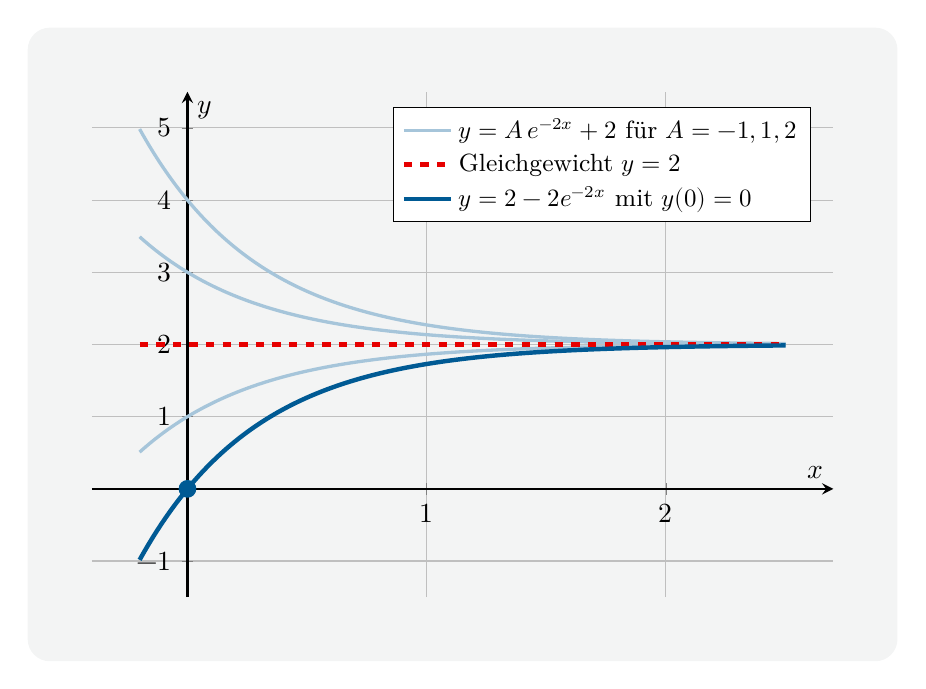
\begin{tikzpicture}[
    show background rectangle,
    background rectangle/.style={fill=my_lightgray, rounded corners=8pt},
    inner frame sep=0.8cm
]
% ---------------------------------------------------------------
%  Loesungen y = A e^{-2x} + 2 der DGL y' + 2y = 4 fuer A = -1, 1, 2,
%  die Gleichgewichtsloesung y = 2 (A = 0) und hervorgehoben die
%  Loesung des AWP y(0) = 0, also A = -2.
%  Werte bei x = -0.2: e^{0.4} = 1.49, also 4.98, 3.49, 0.51, -0.98.
%  axis equal weggelassen: Bei gleicher Skalierung waere das Bild
%  bei y-Werten von -1.5 bis 5.5 und x-Werten bis 2.5 zu hoch.
% ---------------------------------------------------------------
\begin{axis}[
    axis lines = center,
    xlabel = {$x$},
    ylabel = {$y$},
    grid = both,
    axis line style={thick},
    width=11cm, height=8cm,
    xmin=-0.4, xmax=2.7,
    ymin=-1.5, ymax=5.5,
    xtick={1, 2},
    ytick={-1, 1, 2, 3, 4, 5},
    legend pos=north east,
    legend style={font=\small},
    legend cell align=left,
]
\addplot[draw=my_darkblue!35, samples=200, very thick, domain=-0.2:2.5]
    {2*exp(-2*x) + 2};
\addlegendentry{$y = A\,e^{-2x} + 2$ für $A = -1, 1, 2$}
\foreach \A in {-1, 1}{
    \addplot[draw=my_darkblue!35, samples=200, very thick, domain=-0.2:2.5,
        forget plot] {\A*exp(-2*x) + 2};
}
\addplot[draw=my_red, ultra thick, dashed, domain=-0.2:2.5] {2};
\addlegendentry{Gleichgewicht $y = 2$}
\addplot[draw=my_darkblue, samples=300, ultra thick, domain=-0.2:2.5]
    {2 - 2*exp(-2*x)};
\addlegendentry{$y = 2 - 2e^{-2x}$ mit $y(0) = 0$}
\addplot[only marks, mark=*, mark size=3pt, my_darkblue, forget plot]
    coordinates {(0, 0)};
\end{axis}
\end{tikzpicture}
\end{document}
